\chapter{Models@Runtime for the IoT}
\label{ch:MARContiki}
%As presented in chapter \ref{ch:IoT}, Internet of Things systems are typically formed by a myriad of many small interconnected devices.
%This underlying hardware infrastructure raises new challenges in the way we administrate the software layer of these systems.
%Indeed, the limited computing power and battery life of each node combined with the very distributed nature of these systems, greatly adds complexity to distributed software layer management.

As we stated in the previous chapter, the capacity of dynamically deploying and reconfiguring the software layer on the IoT is a crucial feature.
Designing a middleware in the context of the IoT raises scientific challenges.
All the following challenges are related to the limited resources of these nodes and the particular topology of the network that interconnect them.
We address the problem of enabling the deployment of a distributed software layer and its dynamic reconfiguration over a network of nodes featuring very limited resources: memory, processing power, bandwidth communication and energy autonomy.
Therefore, a simple adaptation of an already provided implementation for deployment and reconfiguration in distributed systems would not work.
Indeed, the very scarce resources limits the use of complex approaches \textit{"as is"}, as it was already described in section \ref{sec:dynamicDeploymentDAS}

% limitation of SOTA
To solve this problem, various techniques have been proposed, which were presented in table \ref{tab:deployMethods}. 
As for the full kernel replacement mechanism, which is managed by an automatic tool\cite{hui2004dynamic}, the excessive amount of power needed by this approach seems not to be adapted for a highly dynamic infrastructure such as the IoT.
The approaches making use of virtual machines were already analyzed and it was found that they are not suitable for long-living applications\cite{oliver2014reprogramming}.
Thus, the lack of a deployment manager leveraging kernel modularization using relocation mechanisms, which seems the best way to provide new features and updates, motivates our research to find an automatic and scalable approach to provide such a manager.

Indeed, the previously studied models@runtime approach, and more specifically, the Kevoree meta-model, provides a way to manage the application layer for distributed systems.
As stated in section \ref{sec:distDeployment}, the high resemblance between distributed systems and the IoT, makes the use of such approach a viable solution.
However, the huge differences in computing capacity and energy autonomy between the nodes involved in both scenarios make the implementation of this approach very challenging.
Thus, a direct mapping of Kevoree (the meta-model and its model manipulation tools) cannot be foreseen.

In this chapter, I describe a first approach to implement a new middleware dedicated to IoT devices, in order to enable the management of software deployment and the dynamic reconfiguration of IoT systems.
Our middleware is inspired from the Component Based Systems and the model@runtime paradigm which have been already described in the previous chapter.
Moreover, the implementation of this middleware follows the directions of the existing Kevoree meta-model depicted in \todo{annex or figure?}, which has been adapted to fit IoT devices constraints. 
Our evaluation of these constraints was conducted on several hardware platforms typical of the IoT, in order to establish a reference for the minimum requirements to run such a middleware.
Once an initial research on these IoT platforms was conducted, the proposition of a new one was necessary, since the minimal requirements were not met by the commercially available platforms at that time.
Such platform was an essential part to evaluate our first implementation, and was used to establish the minimum requirements of an execution environment.
Finally, we have conducted the evaluation of our approach on an Internet of Things testbed\cite{Fleury15iotlab} recently available for experimentation.
Our results demonstrates the feasibility of providing a model@runtime middleware for these systems, which can be executed in platforms meeting the requirements already established.
This chapter is concluded by the obtained results on the FIT IoT-Lab testbed, which show the limits of our first approach.

\section{Overview}
\label{sec:MAR_overview}
The Kevoree framework, which was already introduced in subsection \ref{subec:kevoree}, is composed by a meta-model which describes the main parts of a distributed system, coupled with a minimalistic component model.
A typical Java implementation of this meta-model can consists in code generated by using common modeling tools, such as the Eclipse Modeling Framework (EMF)\cite{steinberg2008emf}, resulting in a vast quantity of code representing all the classes and its relationships.
Even if big efforts to reduce the generated code and dependency resolution complexity present in EMF were conducted by Fouquet \textit{et al.} in \cite{fouquet2012eclipse}, the need of a JVM and a big amount of memory still the main inconvenient for its use on the IoT.
Moreover, the principle of a model@runtime lies in the general knowledge of the entire system (the reflected model of the running system), which is present in every participant.
Indeed, the reflected model should be available in memory for its rapid manipulation, thus we can imagine the big quantity of memory needed to represent large models featuring a vast quantity of nodes.
In addition, each node can have instances of one or more components and its parameters, which increase even more the size of the model in memory.
It is then very complex and challenging to provide such a framework on the context of IoT.

\begin{figure}[]
	\centering
	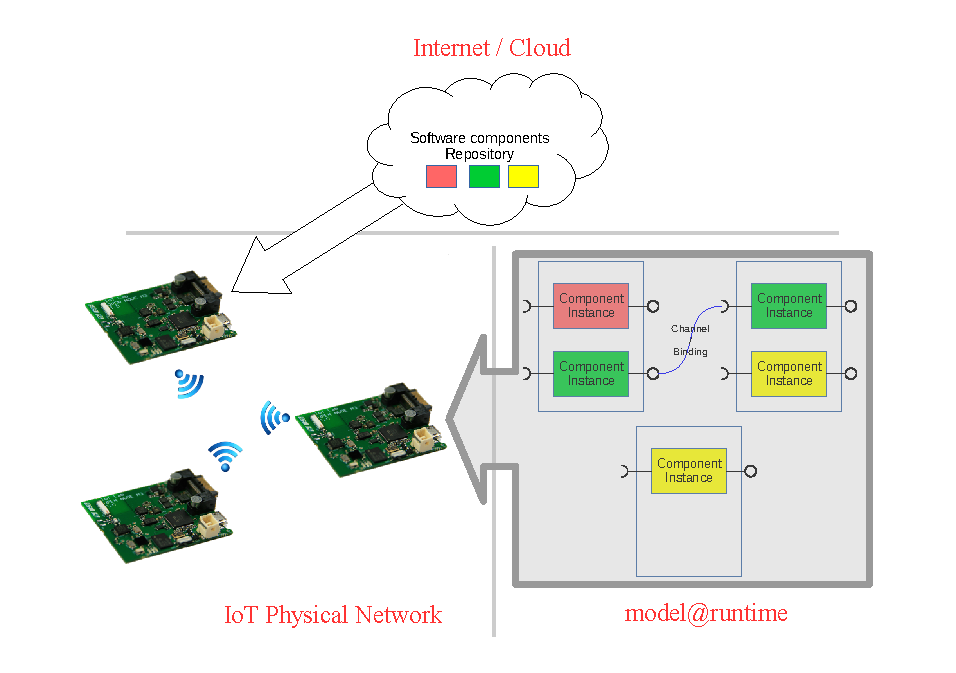
\includegraphics[width=1\columnwidth]{chapters/modelsAtRuntimeContiki.images/MAR_IOT.pdf}
	\caption{A M@R representation for IoT devices.}
	\label{fig:MAR_IOT}
\end{figure}

Our goal is then to provide a middleware that will be present on each node of the IoT system, and will take care of the various tasks imposed by the model@runtime paradigm.
In figure \ref{fig:MAR_IOT} we can appreciate a representation in which three IoT nodes are part of a small network.
This example shows a M@R which is present on the three nodes.
Each node have the knowledge about three available components on the repository, the instances present in the other two nodes and a binding through a channel between two components of different nodes.
Any change of this configuration should be reflected on the model, followed by the dissemination of these changes to the other nodes, and vice-versa, any change on the model will affect the actual node.
Figure \ref{fig:MAR_reconfig} describes the actions taken when a reconfiguration or adaptation is triggered.

\begin{figure}[]
	\centering
	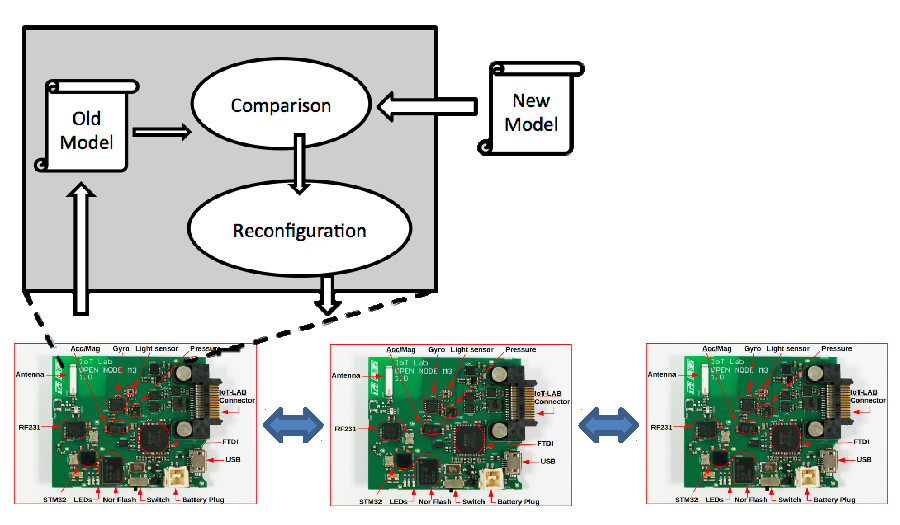
\includegraphics[width=1\columnwidth]{chapters/modelsAtRuntimeContiki.images/MAR_reconfig.pdf}
	\caption{Reconfiguration through a M@R.}
	\label{fig:MAR_reconfig}
\end{figure}

Following the directions presented above, an implementation of this approach on IoT nodes has been conducted, which should be able to have a similar model representation in memory and to enact the adaptation and reconfiguration process on each node.
As we stated before, the exact implementation of the Kevoree M@R approach using the current tools is not possible, due to the IoT node's constraints.
Thus, we will address each constraint and propose an implementation to meet them, while offering a similar behavior and interoperability with the other implementations.
The next section describes how we addressed such constraints.

\section{Kevoree and the IoT}
\label{sec:kevAndIoT}
The Kevoree framework is composed by several parts which provide a complete models@runtime implementation.
The base of this framework is the Kevoree meta-model, which was designed to follow a distributed architecture and a minimalistic component model.
Thus, a first challenge lies in the implementation of such meta-model meeting the programming language and memory constraints.

\subsection{Meeting the memory constraint}
As already discussed in section \ref{sec:MAR_overview}, the Kevoree meta-model can be easily transformed into Java code using a modeling framework.
However, in our case this approach cannot be used.
This is due to two reasons: first, we cannot use high-level languages such as Java and second, we are limited to the C language which can be compiled for the IoT node's architecture already presented in \ref{subsec:smartObjects}.
Moreover, meta-models follow very often an object-oriented approach, which is not defined for procedural languages such as C.
Thus, a direct transformation with this constraints is not worth considering.
However, a similar approach for code generation and modeling tools can be proposed to meet the requirements of a model@runtime approach.
Indeed, the Kevoree Modeling Framework\cite{fouquet2012eclipse} can be adapted to support the generation of C code, in order to provide a fully Kevoree-like middleware for IoT devices.
Even so, the efforts to adapt such a framework raise more and different challenges that are out of the scope for this thesis.
Since our goal is to, first of all, investigate the limits of an IoT node in terms of memory, a manual implementation (transformation) of the meta-model and its modeling tools was made, adapting the concepts to the limited resources of the node.
Indeed, this allows a rapid prototype which can be finely tuned to meet the memory constraints present in IoT devices, in contrast to a code generation approach.

On the typical implementation of Kevoree, a \textit{core} application is embedded in every node. 
This application provides to each system element (node, component, communication channel, groups) an access to the current model, allowing to submit new configurations through new models.
If this \textit{Kevoree Core} receives a new model, it is in charge of the validation, then the adaptation planning and finally the execution of this adaptation.
The set of these stages is carried through a transactional manner.

The model validation is delegated to any system element registered as a \textit{listener}.
Each component, communication channel or node can make use of an interface and be registered on the \textit{core} in charge of the model management.
Once registered, the instance is notified with regard to the different reconfiguration stages.
For this, a \textit{listener} interface can define the following notifications:
\begin{itemize}
	\item \emph{preUpdate} allows to the \emph{listener}s to be notified that an update has been proposed.
	Each \emph{listener} can then validate the proposed configuration.
	\item \emph{preAllUpdate} allows to the \emph{listeners} to be notified that the proposed update has been validated by the set of \emph{listener}.
	\item \emph{postUpdate} allows to the \emph{listeners} to be notified that the update has been applied.
	Each \emph{listener} can then validate that the update does not cause a problem.
	\item \emph{postAllUpdate} allows to the \emph{listeners} to be notified that the update which has been applied was also validated by the set of \emph{listener}s.
	\item \emph{preRollback} allows to the \emph{listeners} to be notified that the update has failed and a rollback to the previous configuration will be carried out.
	\item \emph{postRollback} allows to the \emph{listeners} to be notified that the rollback has been successful.
\end{itemize}
Figure \ref{fig:MAR_modelListener} represents in a state-transition diagram the integrations of \textit{listeners} with the process of \textit{model@runtime}.

\begin{figure}[]
	\centering
	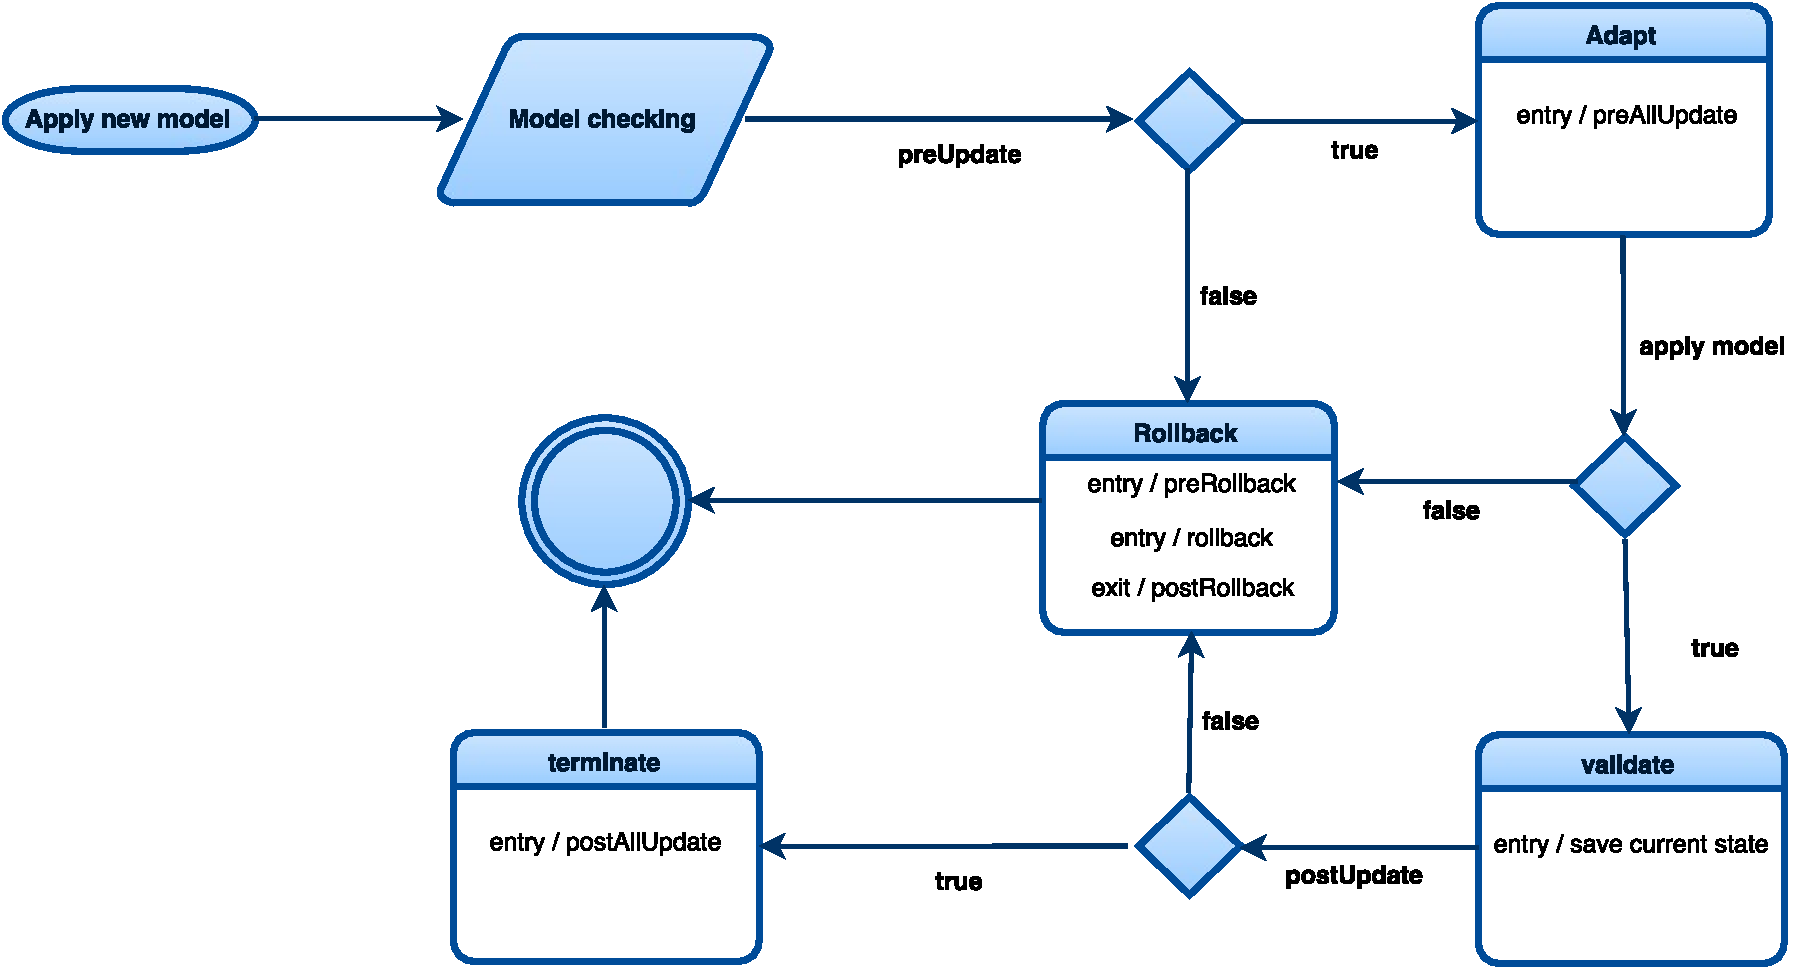
\includegraphics[width=1\columnwidth]{chapters/modelsAtRuntimeContiki.images/ModelListenerStateChart.pdf}
	\caption{State-transition diagram showing the integration of ModelListeners in the M@R process.}
	\label{fig:MAR_modelListener}
\end{figure}

In contrast, our implementation for IoT devices cannot follow the same approach.
Indeed, the model checking and rollback mechanisms require to save the entire model in memory for checking and, if something goes wrong, to bring back the previous model.
This is very memory consuming for our application.
Therefore, only a simple model checking followed by the adaptations execution has been implemented.
Moreover, the implementation of this mechanism for all the system elements (component, communication channel, group) was not necessary for our first prototype.
Thus, only a \textit{ModelListener} is present for the node component, avoiding all the notification process, saving processing time thus energy.
Indeed, in our implementation the node is in charge of the adaptation mechanisms, since for our concerns (an IoT system) nodes are the main component and it can only execute an instance of itself.
This vision contrast with a typical Kevoree implementation, where various \textit{Kevoree Core} can run in a single machine, resulting in several nodes reflected in the model.

In conclusion, our proposition for a Kevoree implementation on IoT devices is conceivable, since we bring the most important features with a very low memory footprint, having only a few limitations.


\begin{figure}[]
	\centering
	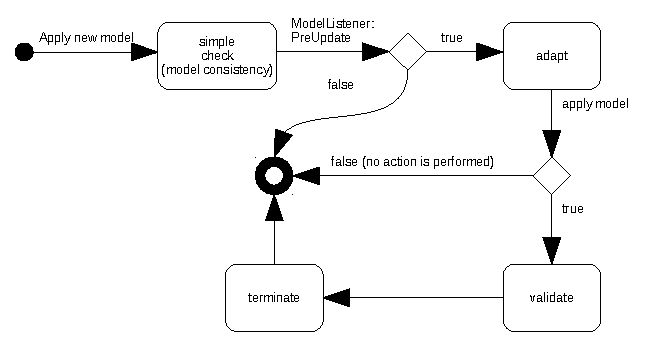
\includegraphics[width=0.85\columnwidth]{chapters/modelsAtRuntimeContiki.images/modelListenerIoT.pdf}
	\caption{State-transition diagram showing the integration of ModelListeners in the M@R process for IoT devices.}
	\label{fig:MAR_modelListenerIoT}
\end{figure}

Figure \ref{fig:MAR_modelListenerIoT} depict the state-transition diagram according to our M@R process for IoT devices.

\subsection{Energy, processing and communication constraints}
Another concern while adapting the Kevoree M@R implementation is the amount of energy needed to run it.
Indeed, an IoT device running on batteries should be able to embed this middleware without a high overhead in terms of energy consumption.
Since the most processor consuming task is the model checking and adaptations execution, a smaller overhead is induced, compared to the traditional approach, thanks to the simplification of such process.
However, it was discussed that the most energy consuming task for an IoT device is the radio communication.
The traditional Kevoree implementation was done having in mind no restrictions for network usage and bandwidth, thus algorithms such as Gossip\cite{fouquet2012dissemination} were used for model dissemination.
The implementation of such a protocol in an IoT device could be very memory consuming, in addition to a high energy consumption while using the network.

Given the energy and memory constraints, a dissemination protocol adapted for IoT devices is then needed.
It results interesting that the already described Deluge protocol\cite{hui2004dynamic} seems to be a good option, since it was developed having in mind the constraints of an IoT device.
As the information to be shared is not as big as an entire firmware, but rather a small serialized file including the model, the needed energy to disseminate a model can be low enough.
Moreover, a compression method using an association table including the most often used keywords has been proposed, reducing the model size by more than a half.
By these means, a small file including the model is shared between all the concerned IoT nodes in the network.


%context
%Based on this principle, IoT dedicated devices have emerged, forming the IoT infrastructure already described in section \ref{sec:IoTInfra}.
%All this new IoT devices form a constellation of many small interconnected objects integrated into houses, building, cities, factory chain, etc.
%Based on this principle, Cyber Physical Systems (CPS) have emerged.CPS are pervasive and long living systems formed by a constellation of many small interconnected devices integrated into houses, building, cities, factory chain, etc. 
%motivation
%In our building automation scenario presented in section \ref{sec:BAScenario}, the described IoT subsystem typically rely on sensor nodes that detect and record data such as presence, temperature, ambient lighting and energy consumption. 
%Thus, the IoT uses sensors to continuously analyse the situation in order to adapt our living environment to match user needs and preferences.
%User wishes may involve different objectives such as comfort, air quality, and energy savings. 
%To go beyond energy management and comfort, building automation systems have to deal with new types of services, depending on the use of the building: fire safety and security management for hotel, indoor air quality control in schools and office buildings, etc. 
%The opportunities of services offered by the IoT and the user preferences are countless and will change over the lifetime of these systems.
%The set of small interconnected devices integrated into buildings can be seen as a computing infrastructure that can host these new services. 
%Consequently the software deployed on these nodes needs to be dynamically reconfigured and re-deployed to meet the evolution of services and user preferences. 


% old sentences
%Consequently comfort and quality are factors of productivity and do not prevent energy savings being achieved.
%To go beyond energy management, building automation systems have to deal with new types of services, depending on the use of the building: fire safety and security management for hotel, indoor air quality control in schools and office buildings etc. 

%problem


%our approach

%plan
%This paper is structured as follows. Section 2 presents the Kevoree component model. Section 3 details the challenges of mapping the model@runtime paradigm to microcontrollers, and explains how we implemented Kevoree on these very limited nodes. Our proposal is evaluated in section 4. Section 5 presents related work and Section 6 gives our conclusion and highlights some perspectives to be addressed in future work.

\section{An empirical study on constrained IoT devices}
The model@runtime paradigm has been mainly investigated in the context of distributed systems. 
These research efforts have been focused on the provision of a comprehensive set of tools to easily deploy, dynamically reconfigure, and disseminate software on a set of distributed computing units.
The current model@runtime tools have been implemented regardless of the specific characteristics and constraints of IoT devices.
In particular, the network topology and the resource constraints of the nodes forming the distributed system have not been taken into consideration.
As a result, state of the art model@runtime tools are not suitable to be used in the context of IoT Systems.
%First, most approaches are relying on the Java language, which does not meet the resource constraints of the computing nodes. 
%Secondly, the size of the model and its distribution among the system are not taking into consideration the limited memory capacity of each node, and their energy constraints.

In \cite{fouquet2012dynamic} $\mu$-Kevoree, the closest effort to port the model@runtime paradigm on the constraints of a Cyber Physical System (CPS) was presented, in which the underlying device is comparable to an IoT device.
Despite the particular attention given to the specific constraints of a Cyber Physical System, this work heavily relies on over the air firmware flashing to support the deployment and reconfiguration of software. 
We consider that relying on firmware flashing to support software deployment constitutes a flaw in the approach because of its energy cost (the complete firmware has to be sent, and if any error occurs, the whole process is restarted).
A second limitation of this approach lies in the fact that each resource constrained node relies on a more powerful node to perform most of his task related to the dynamic reconfiguration (firmware synthesis, reconfiguration decision and so on).
This second limitation is not suitable in the context of a system mainly composed of resource constrained nodes since all the resource constrained nodes have to be managed by bigger nodes.
Pushing this idea further, the management of a CPS composed of a wide number of resource constrained devices and a bigger node, the latter will have to manage all the smaller devices in a centralized management scheme.

Therefore, a new approach implementing a more complete M@R engine has been proposed.
The next section will describe an implementation based on the Kevoree meta-model, together with some tools which allow model manipulation.

\subsection{Our M@R implementation}
\label{subsec:MARImpl}
%Since our work aims to provide a M@R engine for IoT devices, a first implementation should be developed having in mind the programming constraints.
%Taking into account this limitations means that, first of all, we must fit the programming constraints.
In contrast with most of the current implementations of the M@R paradigm, which are intended for high resources machines thus they make use of high-level programming languages, our first implementation should follow a procedural language such as C.
We can justify this by the fact that most of the open source compilers for IoT devices support only this programming language, in addition to C++.
However, C++ applications are difficult to integrate in OSs like Contiki, which is one of the most convenient OS able to run our middleware.
Thus, a first approach has been developed in plain C\footnote{\url{https://github.com/kYc0o/kevoree-c}} following the directions presented in Section \ref{sec:kevAndIoT}.
%This raised big challenges since the object-oriented meta-model representation is very difficult to transform into C structures, knowing that there is no modeling framework supporting such a language.

\begin{table}[]
	\centering
	\caption{Size of a plain C minimalistic Kevoree meta-model implmentation}
	\label{tab:kevoreeC}
	\begin{tabular}{cccccc}
		\texttt{text}   & \texttt{data} & \texttt{bss} & \texttt{dec}    & \texttt{hex}   & \texttt{filename} \\
		\texttt{181997} & \texttt{1448} & \texttt{168} & \texttt{183613} & \texttt{2cd3d} & \texttt{main}        
	\end{tabular}
\end{table}

\begin{figure}[]
	\centering
	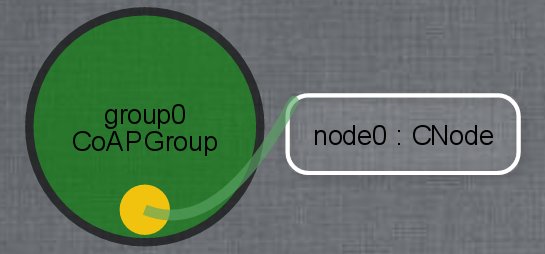
\includegraphics[width=0.55\columnwidth]{chapters/modelsAtRuntimeContiki.images/1stModel.png}
	\caption{Graphical representation of a minimal M@R}
	\label{fig:1stModelC}
\end{figure}

Indeed, our efforts were put into a first manual implementation of the Kevoree meta-model.
The size of the test application which contains a group and a node without components is shown in table \ref{tab:kevoreeC}
A graphical representation of the model can be obtained through the Kevoree Web Editor\footnote{\url{http://editor.kevoree.org/v4/}}, in which a serialized JSON file containing the model can be loaded for edition.
This representation is shown in figure \ref{fig:1stModelC}.

Our firsts results show that approximately 180KB of ROM space (text) are needed for the implementation, while 14KB of RAM (data + bss) were enough for such application.
This test was compiled using the GCC (GNU C Compiler) version 4.9, for a i386 32-bit platform.
Therefore, we need to find an IoT device which fit this minimal requirements.

It is then necessary to characterize the minimum system requirements for an IoT device to implement a full model@runtime middleware, as in hardware capabilities as in execution environment.
This will avoid the use of third party nodes to perform the high level tasks described above.
However, even if a proposed device meet the characteristics to perform such tasks, the trade-offs between energy consumption and the middleware execution should be taken into account.
A general description of needed features to execute the proposed middleware is given in the next subsection.

%\subsection{Needed features of the underlying system}
\subsection{Kevoree-IoT operating system requirements}
Our middleware approach, which is called Kevoree-IoT (in reference to the kevoree-like M@R implementation of our middleware), will need several features from the underlying system.
As we discussed previously, the most common approach used to run applications on IoT devices is bare-metal development followed by firmware flashing into the ROM memory.
Even if this method allows a fine control of the underlying hardware, the development time can be very long and difficult to debug, since abstractions are mostly done only at the hardware level, and does not come to the system level.
As the complexity grows, applications for IoT should be developed without special attention to hardware and system concerns.
Thus, an IoT operating system should be used, in order to leverage its system-level abstractions.
As presented in the state of the art, several IoT operating systems exist, but according to the needed features we should make a choice.
This features are the following:
\begin{enumerate}
	\item \textbf{Network stack implementing basic IP functions (TCP, UDP, HTTP, CoAP).} In order to share a m@r and download software artifacts, IP communication is mandatory, since the goal is to use the Internet to reach devices from different domains.
	\item \textbf{Persistent data handling, preferably a file system.} The method used to represent a m@r is using serialized objects, usually in the JSON format. Thus, a way to store this JSON file should be provided.
	\item \textbf{Dynamic linker and loader, following the third approach presented in section \ref{sec:IoTDeployment}.} A dynamic linker and loader is essential to our approach, since changes in the model containing new software components will trigger the download and instantiation of an artifact, which should be linked and loaded at runtime by the underlying system.
	\item \textbf{Abstractions for attached devices (LEDs, sensors, actuators, etc.).} Although not mandatory, an OS usually carry basic hardware abstractions, providing an easy way to develop applications which need a physical interaction with the external world.
	\item \textbf{Basic OS functionalities such as timers, task scheduler and Inter Process Communication (IPC).} Basic functionalities that are implemented very often by almost any OS.
\end{enumerate}
Given the features presented above, the system which fits all the requirements is the Contiki OS.
Despite the programming model already described as a drawback, Contiki offers all the needed functionalities, as well as a wide community which collaborate very actively in the development and debug of it.
Therefore, we use the ContikiOS\cite{dunkels2004contiki} in order to provide an efficient way to distribute components, since it allows dynamic loading of binary modules.
Contiki includes an implementation of the IPv6 compressed stack, 6loWPAN\cite{rfc4944}, which let us assign directly an IPv6 address. 
This enables a ready to use IoT environment.
We use erbium's\cite{rfc7252} CoAP implementation in order to have a REST engine which is used as a main communication channel between nodes. The dynamic code loading mechanisms are based on a dynamic linker and loader that use the standard ELF object file format\cite{dunkels06runtime}.

However, even if the OS fulfill all the requirements, the computational resources needed by our middleware should be taken into account, in order to find a platform on which we can evaluate our approach.


\subsection{Handling hardware constraints}
%Currently the concept of model@runtime has been applied on top of object oriented languages which offers the required features at the language level to implement the model@runtime layer. 
%The first challenge lies in the fact that Contiki does not support these object oriented languages and thus the design must fit a procedural language such as C.

%The second challenge lies in the very limited resources of the IoT nodes, thus forcing the middleware to meet the memory and CPU constraints. 
%This imposes constraints on the way the model is represented, stored and processed on each node.
%This challenge is particularly important and hard to meet, since many software components are needed to enable the communication in these environments (radio/MAC/IP stack and so on).
Given the challenges already stated in Section \ref{sec:kevAndIoT}, we must test our implementation on real hardware platforms in order to measure the limitation of our approach, as well as its compatibility with the other implementations (Java, Cloud, Android).
Moreover, the energy constraint of each IoT node, together with the mesh topology of the network makes communication in this environments fairly reliable.
This implies the necessity to optimize the way the model and the software are disseminated on the network.

At first glance, our implementation was tested on three different platforms: the \textit{\textbf{zolertia Z1\footnote{\url{http://zolertia.sourceforge.net/wiki/images/e/e8/Z1_RevC_Datasheet.pdf}}, redbee econotag\footnote{\url{http://redwire.myshopify.com/products/econotag-ii}} and wismote\footnote{\url{http://wismote.org/doku.php}}}}, which were widely used for research purposes in the IoT domain.
Unfortunately, none of these platforms was able to meet the space requirements in ROM and RAM to run a minimal model at runtime as shown in figure \ref{fig:1stModelC}.
However, the existence of more powerful microcontrollers, an essential part of an IoT device, shows that typical IoT applications have not exceeded the resources of existing experimentation platforms.
Indeed, only some development kits such as TI's CC2538DK\footnote{\url{http://www.ti.com/tool/cc2538dk}} were available at that time, but its high cost, low availability and poor support gave low acceptance for research purposes.
Thus, the design and construction of a new experimentation platform seemed to be the fastest way to obtain the first results of the implementation, by integrating the latest microcontrollers and peripherals available on the market.
It is worth to consider that this platform was conceived for research and experimentation purposes, and not as an end-user device.

An exhaustive search was conducted to find the latest technologies to build an experimentation IoT device, which fits the requirements already estimated in section \ref{subsec:MARImpl}.
The first step was to find the basic components of such a device.
Taking into account the requirements, an IoT device should embed:
\begin{enumerate}
	\item \textbf{Microcontroller.} A very low-power microcontroller unit is needed to perform the computational processing tasks as well as to store the program code. 
	A huge amount of ROM and RAM is needed at the scale of these devices, thus it is necessary to find a microcontroller with a good trade-off between energy consumption and memory size.
	\item \textbf{Communication interface.} Communication is the main task that will perform our device, since it is mandatory for IoT environments.
	A radio interface implementing the widely used IEEE 802.1.5.4 standard\cite{ieee802.15.4} is then necessary to communicate in an interoperable way with other devices.
	An ultra-low energy consumption is also important, since communication is the most energy consuming task.
	\item \textbf{External flash memory.} Storage for data is a very useful feature for an IoT device. It can serve as persistent data storage for logging and data collection from sensors, as well as updates and eventually new firmwares.
	\item \textbf{Sensors and actuators.} In order to collect experimentation data, some sensors should be embedded on the device, the most common being temperature, humidity and position.
	Indicator LEDs are also commonly present in these devices, to provide visual signs such as function status (ON/OFF) or current communication.
	\item \textbf{Ports for external devices.} An easy way to connect third party devices allows a dynamic behavior, since we can connect other sensors, actuators and devices which cannot be present internally on the device.
	Such devices should be connected using standard interfaces, such as I2C and SPI.
	General Purpose Inputs/Outputs (GPIO) are also widely used, either as digital or analog interfaces.
	\item \textbf{Battery capabilities.} An IoT device is very often used in environments where a constant power source is not present.
	Thus, work on batteries is a very useful feature to test energy consumption while adding flexibility of placement.
\end{enumerate}

Given these features, it was then necessary to integrate several components in order to build the required IoT device.
We put special attention to the most critical components, which are the microcontroller, the external flash memory and the battery controller.
Regarding the radio transceiver and the other peripherals, there are no huge differences between the most commonly used, for instance, the ones used in the previously tested devices.
The specific conception of the platform will be described in the next subsection.

\subsection{Towards a new IoT device}

Several low-power microcontroller architectures were available at the time of our first M@R implementation, such as TI MSP430, Atmel AVR, Microchip PIC and ARM Cortex-M, just to mention the most common ones.
Since our middleware minimum memory requirements were tested on 16-bit MSP430 microcontrollers (Zolertia's Z1 and Arago's WiseMote) finding a huge scarcity of memory, 32-bit architectures were the target of our scope.
Indeed, ARM Cortex-M microcontrollers offer only 32-bit RISC architectures, which are widely used both in research and industry.
Thus, the first step was to select an ARM Cortex-M microcontroller fitting our memory and energy consumption requirements.
The ST Microelectronics STM32 family of microcontrollers offers a wide range of devices with different processor speeds and memory sizes.
\begin{figure}[]
	\centering
	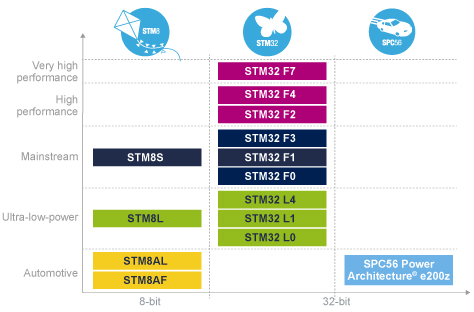
\includegraphics[width=0.70\columnwidth]{chapters/modelsAtRuntimeContiki.images/STM32.jpg}
	\caption{STM32 Microcontroller family}
	\label{fig:STM32}
\end{figure}
Figure \ref{fig:STM32} shows the STM32 family applications and available solutions for each one.

At the time of this search, ultra-low-power solutions (STM32L) were not available, thus our possibilities were in the STM32F range, excluding the F7 which was also released recently.

\begin{table}[]
	\centering
	\caption{Comparison between STM32F microcontrollers}
	\label{tab:STM32F}
	\begin{tabular}{c|cccc}
		Microcontroller & Speed (MHz) & RAM (KB) & ROM (KB) & \begin{tabular}[c]{@{}c@{}}Consumption \\ at max. speed (mA)\end{tabular} \\ \hline
		STM32F0         & 48          & 32       & 256      & 22                                                                        \\
		STM32F1         & 72          & 96       & 1024     & 68                                                                        \\
		STM32F3         & 72          & 80       & 512      & 61.5                                                                      \\
		STM32F2         & 120         & 128      & 1024     & 49                                                                        \\
		STM32F4         & 180         & 256      & 2048     & 98                                                                       
	\end{tabular}
\end{table}

Since our goal is to build a device on which our experimentations could be executed on a more flexible way (without caring about memory requirements), it is preferable to use a microcontroller featuring the highest memory capabilities, both in ROM and RAM, over energy consumption.
Moreover, these kind of devices are able to change the processor speed as needed, thus reducing the energy consumption.
Therefore, the STM32F4 microcontroller was used as the core of our IoT device.
Table \ref{tab:STM32F} shows a comparison between the available microcontrollers, featuring the maximum processor speed, RAM and ROM, followed by the current consumption in such configuration.

As for the power scheme, given the capabilities of the selected microcontroller, a power source between 1.8V and 3.6V is required.
Indeed, a first approach to power the device is the use of an USB port, which delivers around 5V.
Thus, a 5V to 3.3V (the recommended tension) is required.
In contrast, when the device is needed to run on batteries, the supplied voltage will change.
The most common batteries available on the market provide between 1.5V (AA, AAA) and 3V (CR3032), which is in the acceptable range.
A couple of AA batteries connected in series is the most standard array to power IoT devices, delivering 3V, enough for our device.
However, a wide set of peripherals such as sensors and actuators work very often at 5V.
Therefore, it was necessary to add a DC to DC converter, coupled with an automatic power selector which detects when the device is powered either by USB or batteries.
This allows to use any power scheme without decreasing performance or peripherals compatibility.

\begin{table}[]
	\scriptsize
	\centering
	\caption{IoT Platforms comparison}
	\label{tab:IoTPlatfComp}
	\begin{tabular}{cccccccc}
		\textbf{}                                                                               & \textbf{\begin{tabular}[c]{@{}c@{}}Speed \\ (MHz)\end{tabular}} & \textbf{\begin{tabular}[c]{@{}c@{}}RAM \\ (KB)\end{tabular}} & \textbf{\begin{tabular}[c]{@{}c@{}}ROM \\ (KB)\end{tabular}}                               & \textbf{\begin{tabular}[c]{@{}c@{}}External \\ flash (MB)\end{tabular}} & \textbf{\begin{tabular}[c]{@{}c@{}}Radio \\ transceiver\end{tabular}} & \textbf{Peripherals}                                                                                    & \textbf{\begin{tabular}[c]{@{}c@{}}Embedded\\ Sensors\end{tabular}}                                \\ \cline{2-8} 
		\multicolumn{1}{c|}{\textbf{\begin{tabular}[c]{@{}c@{}}Zolertia \\ Z1\end{tabular}}}    & \multicolumn{1}{c|}{16}                                         & \multicolumn{1}{c|}{8}                                       & \multicolumn{1}{c|}{96}                                                                    & \multicolumn{1}{c|}{2}                                                  & \multicolumn{1}{c|}{CC2420}                                           & \multicolumn{1}{c|}{\begin{tabular}[c]{@{}c@{}}UART, I2C\\ Phidgets \\ (USB only),\\ GPIO\end{tabular}} & \multicolumn{1}{c|}{\begin{tabular}[c]{@{}c@{}}3 axis acc.\\ and\\ temperature\end{tabular}}       \\ \cline{2-8} 
		\multicolumn{1}{c|}{\textbf{\begin{tabular}[c]{@{}c@{}}Arago's\\ WisMote\end{tabular}}} & \multicolumn{1}{c|}{25}                                         & \multicolumn{1}{c|}{16}                                      & \multicolumn{1}{c|}{256}                                                                   & \multicolumn{1}{c|}{8}                                                  & \multicolumn{1}{c|}{CC2520}                                           & \multicolumn{1}{c|}{\begin{tabular}[c]{@{}c@{}}UART, I2C,\\ Phidgets, \\ GPIO\end{tabular}}             & \multicolumn{1}{c|}{\begin{tabular}[c]{@{}c@{}}3 axis acc.\\ light and\\ temperature\end{tabular}} \\ \cline{2-8} 
		\multicolumn{1}{c|}{\textbf{\begin{tabular}[c]{@{}c@{}}Redbee\\ econotag\end{tabular}}} & \multicolumn{1}{c|}{26}                                         & \multicolumn{1}{c|}{96}                                      & \multicolumn{1}{c|}{\begin{tabular}[c]{@{}c@{}}N/A\\ (device run\\ from RAM)\end{tabular}} & \multicolumn{1}{c|}{128 (KB)}                                           & \multicolumn{1}{c|}{Integrated (SoC)}                                 & \multicolumn{1}{c|}{GPIO}                                                                               & \multicolumn{1}{c|}{N/A}                                                                           \\ \cline{2-8} 
		\multicolumn{1}{c|}{\textbf{\begin{tabular}[c]{@{}c@{}}DiverSE\\ Board\end{tabular}}}   & \multicolumn{1}{c|}{180}                                        & \multicolumn{1}{c|}{256}                                     & \multicolumn{1}{c|}{2048}                                                                  & \multicolumn{1}{c|}{16}                                                 & \multicolumn{1}{c|}{CC2520}                                           & \multicolumn{1}{c|}{\begin{tabular}[c]{@{}c@{}}UART (x2), \\ I2C\\ Phidgets, \\ GPIO\end{tabular}}      & \multicolumn{1}{c|}{N/A}                                                                           \\ \cline{2-8} 
	\end{tabular}
\end{table}

Thus far, the main required features for our device are met.
A comparison between the previously tested platforms and ours is given in table \ref{tab:IoTPlatfComp}, showing the most common useful features.
Details about the other components such as the radio transceiver and the external flash memory can be found in \todo{annex X.}
	
An already ported Contiki version\footnote{\url{https://github.com/vedderb/contiki}} for a very similar device was the base of our Contiki port, which provided a basic hardware abstraction layer for the radio interface and some I/O drivers.
The rest of the drivers were developed according to the platform hardware design.
Once the porting completed the next step was to test our middleware on such platform.
To do that, a Kevoree-IoT application should be developed, using this new Contiki port.


\subsection{Kevoree-IoT Contiki implementation}
\label{subsec:kevoreeContikiImpl}
In this subsection we present our initial result towards the design of a middleware which will offer the functionalities of model@runtime over the previously conceived IoT device. 
%Porting the concept of model@runtime on IoT devices will enable a continuous management of the deployed software.
This middleware will give a development framework for the  applications development on top of these systems, and will provide the runtime infrastructure to support the deployment and dynamic reconfiguration of these applications.

%As illustrated in figure \ref{fig:ContributionOverview}, our goal is to provide a middleware that will be present on each node of the system, and will take care of the various tasks imposed by the model@runtime paradigm.
%More specifically, our middleware will be in charge of:
%\begin{enumerate}
%	\item Receiving new models that define the new targeted state of the system,
%	\item Defining the set of local adaptations that are needed to reach this new state,
%	\item Enacting the various local adaptations produced by the previous step.
%\end{enumerate} 

%The set of local adaptations enables the dynamic reconfiguration and may download new software artifacts, instantiate or remove components and channels used to bind them, or reconfigure the value of any attribute.

%\begin{figure}[htb]
%	\centering
%	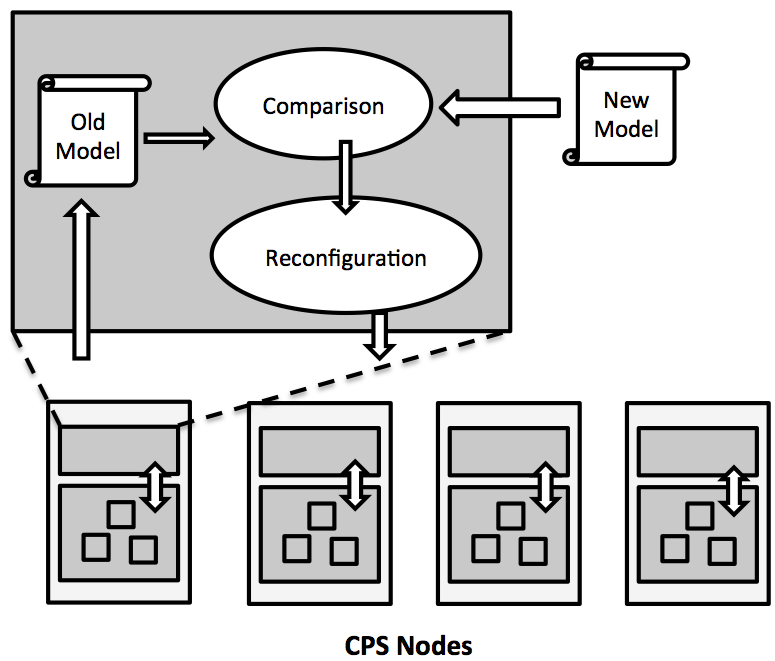
\includegraphics[width=0.7\columnwidth]{chapters/modelsAtRuntimeContiki.images/Contribution_Overview.png}
%	\caption{An overview of model@runtime for IoT devices} \label{fig:ContributionOverview}
%\end{figure}

Based on the Kevoree-C implementation already described in subsection \ref{subsec:MARImpl}, the needed Contiki application was developed and tested in our platform.
The first implementation\footnote{\url{https://github.com/kYc0o/kevoree-contiki}} is done using the version 4 of the Kevoree meta-model, which is depicted in annex \todo{X}.
This meta-model has been mapped into C code as a Contiki application.
We were able to add nodes, components, groups and channels, and bind them through the Kevoree editor by loading a generated JSON file.

\begin{table}[htb]
	\centering
	\caption{Size of a minimalistic Contiki application usign Kevoree-IoT}
	\label{tab:kevoreeContiki}
	\begin{tabular}{cccccc}
		\texttt{text}   & \texttt{data} & \texttt{bss} & \texttt{dec}    & \texttt{hex}   & \texttt{filename} \\
		\texttt{215228} & \texttt{3508} & \texttt{14896} & \texttt{233632} & \texttt{390a0} & \texttt{er-example-server.stm32-diverSE}        
	\end{tabular}
\end{table}

Our firsts results showed that our implementation was able to run on our experimentation device.
This first firmware contains the Contiki OS kernel, device drivers, a CoAP web server and the Kevoree-IoT middleware.
The memory size of this firmware is shown in table \ref{tab:kevoreeContiki}.

Once our middleware was tested in our experimental platform, we needed to test it at large scale.
This needs a large infrastructure with several devices where a basic experiment using our middleware can be executed.
Indeed, the manufacturing of several of our devices was our first option.
However, since the manufacturing of the firsts devices was made by hand, build some other needed a huge amount of time, and can be very costly.
Therefore, a search for large-scale testbeds for the IoT was done.
The next section will describe the found platform and its characteristics, which were analyzed in order to find if they met our requirements.

\section{FIT IoT-Lab: A large-scale testbed for the IoT}
At the time our experimentation a testbed existed at the INRIA Rennes center, where our research team is based.
A Wireless Sensor Network called Senslab\cite{des2011senslab}, formed by 256 devices was deployed in a center's cellar.
This WSN offered wireless sensors of similar characteristics as the Z1 platform, which was already described.
Thus, the minimum requirements to run our middleware were not met by these WSN's devices.
However, an extension of such testbed was done recently, adding new experimentation platforms.
This new platform, called FIT IoT-Lab\cite{Fleury15iotlab}, featured new devices of a similar architecture as ours.
Indeed, two more powerful nodes were added to the testbed: the M3 node and the A8 node, enabling IoT capabilities.

\begin{figure}[htb]
	\centering
	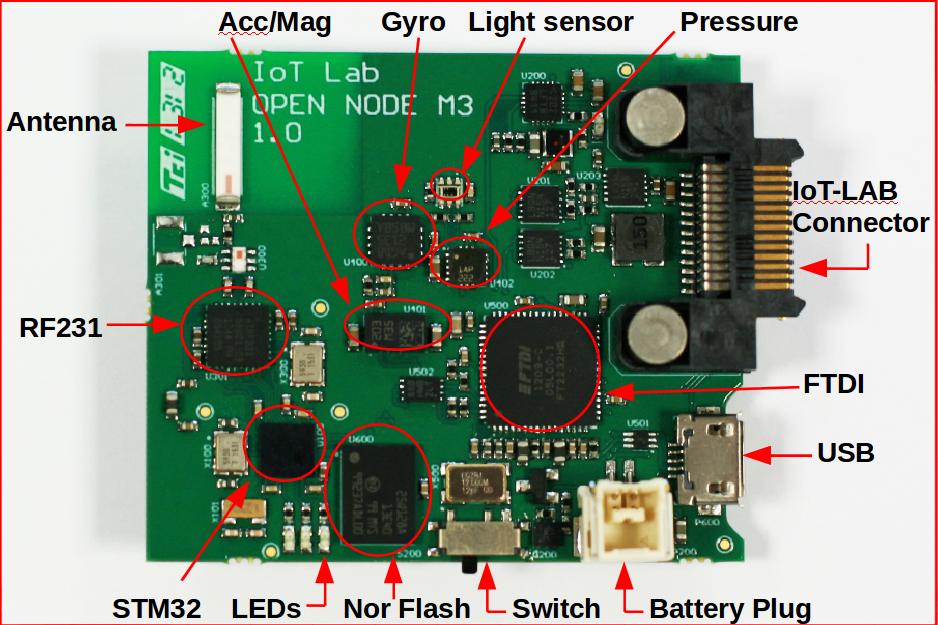
\includegraphics[width=0.7\columnwidth]{chapters/modelsAtRuntimeContiki.images/m3opennode.png}
	\caption{The FIT-IoT Lab M3 Open Node} \label{fig:M3OpenNode}
\end{figure}

Figure \ref{fig:M3OpenNode} presents the M3 Open Node, an IoT device with very similar characteristics of the one from our design.
This device features a STM32F1 Cortex-M3 microcontroller, with 512KB of ROM and 64KB of RAM.
External sensors are available, as well as 3 LEDs.
The communication is handled by an AT86RF231 radio, implementing the standard IEEE 802.15.4, typical of IoT devices.
This combination seems suitable for our experiments, since our firsts results in table \ref{tab:kevoreeContiki} showed that around 200KB of ROM and 16KB of RAM were enough to run a minimal implementation of our middleware.
In addition, a Contiki port for this device was already available, facilitating the integration of our existing implementation for Contiki.
However, two important features lacked in this port: the low-level interface for the Contiki File System (CFS) and the relocation operations needed by the Contiki ELF loader.

Given the importance of these features for the correct implementation of our middleware, it was necessary to extend the testbed capabilities to add support for the CFS and the ELF loader.
The next subsection will give details about the code contribution provided for the IoT-Lab testbed, in order to have a complete IoT platform able to run our middleware and ready for our large-scale tests.

\subsection{Extending the FIT IoT-Lab testbed}
As stated previously, two missing features were detected in the Contiki port made for this testbed.
The first one was the implementation of a low-level interface necessary for the Contiki File System.
This driver make use of low-level functions to read, write and erase the flash memory embedded on the M3 node.
Therefore, this functionality is necessary to leverage the high-level abstractions provided by the CFS, which are a very useful approach to manipulate files into the flash memory, also needed by the ELF loader.

\subsubsection{File system driver implementation}
The definitions and porting instructions for CFS can be found on the wiki page of the Contiki main repository\footnote{\url{https://github.com/contiki-os/contiki.git}}.
A brief description of the file system is given as follows:

\begin{citeverbatim}
	Contiki provides a set of file systems for using various kinds of storage devices in resource-constrained systems. 
	All of these file systems implement a subset of the Contiki File System (CFS) interface, and two of them provide the full functionality: CFS-POSIX and Coffee.
	CFS-POSIX is used in Contiki platforms that run in native mode. 
	It uses direct calls to the POSIX file API that is provided by the host operating system. 
	Coffee, on the other hand, is primarily aimed at sensor devices that are equipped with flash memories or EEPROM.
\end{citeverbatim}

As we can deduce, we aim to port the Coffee file system, since our platform is a resource constrained device embedding a flash memory.
Thus, the porting instructions state that the first step is to provide information about the external memory.
This is done through the \texttt{cfs-coffee-arch.h} file, which in our case was created as shown in listing \ref{lst:flashIface}
\lstset{language=C,
	basicstyle=\ttfamily\scriptsize,
	keywordstyle=\color{blue}\ttfamily,
	stringstyle=\color{red}\ttfamily,
	commentstyle=\color{gray}\ttfamily,
	breaklines=true,
	captionpos=b
}
\begin{lstlisting}[language=C, caption=Contiki header for external memory features, label=lst:flashIface]
/*** N25Q128 Memory Organization
The memory is organized as:
16,777,216 bytes (8 bits each)
256 sectors (64 Kbytes each)
In Bottom and Top versions: 8 bottom (top) 64 Kbytes boot sectors with 16 subsectors
(4 Kbytes) and 248 standard 64 KB sectors
65,536 pages (256 bytes each)
64 OTP bytes located outside the main memory array
Each page can be individually programmed (bits are programmed from 1 to 0).
The device is Sector or Bulk Erasable (bits are erased from 0 to 1) but not Page Erasable.
Subsector Erase is allowed on the 8 boot sectors (for devices with bottom or top architecture).

*/
//Total size of the External Flash Memory in the M3 node
#define COFFEE_XMEM_TOTAL_SIZE_KB       16384UL

/* Coffee configuration parameters. */
#define COFFEE_SECTOR_SIZE   	65536UL
#define COFFEE_PAGE_SIZE       	256UL
#define COFFEE_START            0
#define COFFEE_SIZE             (COFFEE_XMEM_TOTAL_SIZE_KB * 1024UL - COFFEE_START)
#define COFFEE_NAME_LENGTH      32
#define COFFEE_MAX_OPEN_FILES   6
#define COFFEE_FD_SET_SIZE      8
#define COFFEE_LOG_TABLE_LIMIT 	256
#define COFFEE_DYN_SIZE         16*1024
#define COFFEE_LOG_SIZE         8*1024

#define COFFEE_MICRO_LOGS       1

/* Flash operations. */
#define COFFEE_WRITE(buf, size, offset)                \
xmem_pwrite((char *)(buf), (size), COFFEE_START + (offset))

#define COFFEE_READ(buf, size, offset)                \
xmem_pread((char *)(buf), (size), COFFEE_START + (offset))

#define COFFEE_ERASE(sector)                    \
xmem_erase(COFFEE_SECTOR_SIZE, COFFEE_START + (sector) * COFFEE_SECTOR_SIZE)
\end{lstlisting}
We can appreciate that a wrapper to access the external flash is provided by the functions \texttt{xmem\_*}, in order to isolate the platform functions from the Contiki functions.

The second step to achieve the implementation of the low-level interface was to look at the Hardware Abstraction Layer (HAL) already provided with the platform's code.
This HAL is included in a separated repository called \textit{openlab}\footnote{\url{https://github.com/iot-lab/openlab.git}}.
Within this repository, all the low-level drivers providing functions to manipulate every piece of the embedded system are included.
Our concern is to identify those related to the SPI Flash memory.
Indeed, several functions to make use of the flash memory were available, including:
\begin{enumerate}
	\item \texttt{\textbf{void n25xxx\_read\_id(uint8\_t *id, uint16\_t len):}} Reads the flash chip ID which contains the manufacturer ID, the device ID and an unique ID.
	\item \texttt{\textbf{void n25xxx\_read(uint32\_t address, uint8\_t *buf, uint16\_t len):}} Reads a given amount of data from the flash starting anywhere in the flash.
	\item \texttt{\textbf{n25xxx\_write\_enable()}} and \texttt{\textbf{n25xxx\_write\_disable():}} Enable/Disable writing on the flash.
	This function must be called before/after each write operation.
	\item \texttt{\textbf{void n25xxx\_write\_page(uint32\_t address, uint8\_t *buf):}} This function writes the content of a buffer to a given flash page.
	The write must be enabled before calling this function.
	\item \texttt{\textbf{void n25xxx\_erase\_subsector(uint32\_t address):}} Erases a given sub-sector of the flash, a sub-sector is composed of 16 pages (i.e. 4096 bytes).
	The write must be enabled before calling this function.
	\item \texttt{\textbf{void n25xxx\_erase\_sector(uint32\_t address):}} Erases a given sector of the flash, a sector is composed of 16 sub-sectors (i.e 256 page or 65536 bytes).
	The write must be enabled before calling this function.
	\item \texttt{\textbf{void n25xxx\_bulk\_erase():}} This function erases the entire flash.
	The write must be enabled before calling this function.
	\item \texttt{\textbf{uint8\_t n25xxx\_read\_status(void):}} Read the flash status register.
	
	Additionally, three more functions were added to this HAL in order to have full control over the flash memory, needed by the Contiki low-level interface.
	
	\item \texttt{\textbf{void \_n25xxx\_cs\_clear(void)}} and \texttt{\textbf{void \_n25xxx\_cs\_set(void):}} Chip select clear/set allowing to turn on/off an SPI device.
	\item \texttt{\textbf{uint8\_t \_n25xxx\_rw\_byte(uint8\_t byte):}} Allows to read only one byte at once.
	The CS must be set/cleared after each use of this function.
\end{enumerate}
With the use of this functions, the next step was to map them to the Contiki's needed interface.
The full code of the Contiki's wrap functions mapped to the openlab's platform functions is available at the main repository\footnote{\url{https://github.com/iot-lab/contiki/blob/master/platform/openlab/dev/xmem.c}} of the Contiki port for IoT-Lab. \todo{should I use an annex instead?}

The second missing feature is the relocation functions for the embedded ARM Cortex-M3 CPU, used by the Contiki ELF loader in order to find the correct addresses of the symbols provided by the OS.
Indeed, the ELF loader is the main feature used to add new modules to the kernel or update its existing features.

\subsubsection{Runtime address relocation for ARM Cortex-M3 platforms}
As presented in section \ref{sec:IoTDeployment}, we have studied the different methods to add new modules into a running IoT device.
The method used by the Contiki ELF loader is the relocatable code.
This approach needs to relocate the temporary addresses given to the unresolved symbols of a new module, in order to get access to the needed functions provided by the OS.

Since the use of the Contiki ELF loader involves two aspects, a prepared firmware able to load new modules and the new modules themselves, modifications to the compilation routines should be provided for both artifacts.
As described in the Contiki wiki\footnote{\url{https://github.com/contiki-os/contiki/wiki/The-dynamic-loader\#Preparing_a_Firmware_for_ELF_Loading}}, a firmware able to load new modules should be prepared as follows:
\begin{citeverbatim}
	The firmware must be prepared with a symbol table to able to load ELF modules dynamically.
	This three-step process ensures that all available symbols in the firmware are also visible in the symbol table, along with a pointer to their address.
	
	\texttt{make <firmware-name>} \\
	\texttt{make CORE=<firmware-name> <firmware-name>} \\
	\texttt{make CORE=<firmware-name> <firmware-name>} \\
\end{citeverbatim}
Thus, compilation instructions for the \texttt{CORE} variable must be provided.
Since they are CPU specific, they must be added in the Makefile for this specific platform.
\\
\lstset{language=make,
	basicstyle=\ttfamily\scriptsize,
	keywordstyle=\color{blue}\ttfamily,
	stringstyle=\color{red}\ttfamily,
	commentstyle=\color{gray}\ttfamily,
	breaklines=true,
	captionpos=b
}
\begin{lstlisting}[language=make, caption=Compilation settings to create a proper symbol table, label=lst:make4Symbols]
ifdef CORE
.PHONY: symbols.c symbols.h
symbols.c:
	$(NM) $(CORE) | awk -f $(CONTIKI)/tools/mknmlist > symbols.c
else
symbols.c symbols.h:
	cp ${CONTIKI}/tools/empty-symbols.c symbols.c
	cp ${CONTIKI}/tools/empty-symbols.h symbols.h
endif
\end{lstlisting}

Listing \ref{lst:make4Symbols} shows the instructions to create a symbol table for the M3 platform, including all the functions used in the base firmware.
These symbols are created using the \texttt{arm-none-eabi-nm} command to extract all the symbol's names from the main firmware, and with the aid of a Contiki tool called \texttt{mknmlist} a source code file is generated where all used symbols are declared.
Finally, this source code is compiled and linked to the main firmware.
On the other hand, if the \texttt{CORE} variable is not set, a predefined source file without the symbols is copied to be compiled with the main firmware.

As for the creation of new ELF modules, the Contiki dynamic linker and loader\cite{dunkels06runtime} depends strongly on the relocation methods supported by the CPU architectures for which the module is being compiled.
Since our implementation is based on an ARM architecture, we need to provide the relocation functions for this platform.
Indeed, ARM offers the processor-specific definitions in the \textit{ELF for the Application Binary Interface (ABI) for the ARM architecture}\footnote{\url{http://infocenter.arm.com/help/topic/com.arm.doc.ihi0044e/IHI0044E_aaelf.pdf}} document.
This document specifies the way of an ELF binary should be produced by a compiler, including the relocation types.
Thus, this information should be used to implement a dynamic linker which will be in charge of the relocation process for unresolved symbols present in the new module.
For the ARM architecture, more than 100 relocation types exist, but just a few operations still relevant.
We will focus in only 3 types of relocation, which were present in most of the examples we compiled.
These relocation types are presented in table \ref{tab:relocTypes}.

\begin{table}[htb]
	\centering
	\caption{Relocation types compatible with our loader}
	\label{tab:relocTypes}
	\begin{tabular}{|c|c|c|c|c|}
		\hline
		\textbf{Code} & \textbf{Name}       & \textbf{Type} & \textbf{Class} & \textbf{Operation} \\ \hline
		2             & R\_ARM\_ABS32       & Static        & Data           & (S + A) | T        \\ \hline
		10            & R\_ARM\_THM\_CALL   & Static        & Thumb32        & ((S + A) | T) – P  \\ \hline
		30            & R\_ARM\_THM\_JUMP24 & Static        & Thumb32        & ((S + A) | T) – P  \\ \hline
	\end{tabular}
\end{table}

We can appreciate that type 10 and 30 have the same operation.
The following nomenclature is used for the operation:
\begin{itemize}
	\item \textbf{S} (when used on its own) is the address of the symbol.
	\item \textbf{A} is the addend for the relocation.
	\item \textbf{P} is the address of the place being relocated (derived from r\_offset).
	\item \textbf{T} is 1 if the target symbol S has type STT\_FUNC and the symbol addresses a Thumb instruction; it is 0 otherwise.
\end{itemize}

Therefore, we need to implement only 2 types of relocations.
These two types of relocation depends on the information provided by a compatible ELF file, which is first parsed by the Contiki ELF loader.
The requirements of an ELF module handled by the Contiki ELF loader are stated on the Contiki's wiki, as following:

\begin{citeverbatim}
	An ELF file consists of a header followed by a set of sections which typically include at least a section for binary code (\texttt{.text}), a section for statically allocated data with pre-assigned values (\texttt{.data}), and a section for zero-initialized data (\texttt{.bss}).
	Additionally, each symbol is represented in a symbol table (\texttt{.symtab}), and strings are stored in a string table (\texttt{.strtab}). 
	For a file to be accepted by Contiki's ELF loader, it must contain at least the sections listed above. 
\end{citeverbatim}

In order to produce an ELF file compatible with this characteristics, a special method of compilation is provided by Contiki.
Indeed, the Contiki's documentation provide a generic method to produce a Contiki ELF module (CE), as stated below:

\begin{citeverbatim}
	Contiki's build system includes an easy method to create modules that can be loaded into a running Contiki system.
	Simply compile the program with the suffix .ce, as shown below. 
	The suffix instructs the make program to compile an ELF file from a C source file. 
	The object module is stripped from unneeded symbols. 
	The .co suffix works similarly, but does keeps unneeded symbols in the ELF file. 
	
	\texttt{cd example/hello-world} \\
	\texttt{make TARGET=sky hello-world.ce}
\end{citeverbatim}

This method makes use of Contiki's predefined compiler flags that should produce a compatible ELF file.
However, such flags are intended mostly for MSP430 architectures.
We have experimented these default flags for the CE compilation and it was found that several other sections were present in the ELF file.
These "extra" sections contained needed information about the module, and were skipped by the ELF loader.
Thus, specific compilation mechanisms shown on listing \ref{lst:make4CELF} have been proposed to solve this problem.
\\
\lstset{language=make,
	basicstyle=\ttfamily\scriptsize,
	keywordstyle=\color{blue}\ttfamily,
	stringstyle=\color{red}\ttfamily,
	commentstyle=\color{gray}\ttfamily,
	breaklines=true,
	captionpos=b
}
\begin{lstlisting}[language=make, caption=Compilation instructions to generate an ARM ELF file., label=lst:make4CELF]
CUSTOM_RULE_C_TO_CE = "defined"
%.ce: %.c
	@# Requires '-DAUTOSTART_ENABLE' to be loaded
	$(CC) $(CFLAGS) $(OPENLAB_INCLUDE_PATH) -DAUTOSTART_ENABLE -c $< -o $*.o
	$(GCCPREFIX)-ld -r -T $(OPENLAB)/merge-segments.ld $*.o -o $@
	$(STRIP) --strip-unneeded -g -x $@
\end{lstlisting}

As we can appreciate, a special linking phase (triggered by the \texttt{-ld} flag) using a linker script was needed to merge the extra sections generated by the standard compilation phase, followed by the stripping mechanism for unneeded symbols (mostly debug symbols).
This script consisted in merge all \texttt{.text, .data, .rodata} and \texttt{.bss} related sections into only one.
For instance, without this script, a hello world example generated the following sections:

\begin{listing}
	\texttt{.text.process\_thread\_hello\_world\_process} 
	\texttt{.rel.text.process\_thread\_hello\_world\_process}
	\texttt{.rel.data.hello\_world\_process}
	\texttt{.rodata.autostart\_processes}
	\texttt{.rel.rodata.autostart\_processes}
	\texttt{.rodata.str1.1}
\end{listing}

This are the standard sections generated by the \texttt{arm-none-eabi-gcc} compiler without the linking phase where the script is executed.
Since sections other than the required by the loader are ignored, the loading attempt will result in an unsuccessful module execution.
Details about the script are shown in listing \ref{lst:script4CELF}.

Once the correctness of the ELF file is validated by the loader, a relocation phase is conducted.
This makes use of the ELF loader internals, which should be defined by the platform.
These internals are described by Contiki as follows:
\begin{citeverbatim}
	Each CPU architecture in Contiki that supports ELF loading implements a set of architecture-dependent functions. 
	The table \ref{tab:loaderFunc} shows the API that needs to be implemented in order to support ELF loading. 
	These include functions allocate RAM for data (\texttt{elfloader\_arch\_allocate\_ram()}), allocate read-only memory (ROM) for code (\texttt{elfloader\_arch\_allocate\_rom()}), write to the allocated ROM (\texttt{elfloader\_arch\_write\_rom()}), and relocate addresses in the ROM (\texttt{elfloader\_arch\_relocate()}). 
	The relocation information is stored in objects of type \texttt{struct elf32\_rela}, which is defined below in listing \ref{lst:ELFreloc}. 
	In this structure, \texttt{r\_offset} indicates the location to be relocated, \texttt{r\_info} specifies the relocation type and symbol index, and \texttt{r\_addend} is the value to add when relocating an address in \texttt{elfloader\_arch\_relocate()}.
\end{citeverbatim}

\begin{table}[htb]
	\centering
	\scriptsize
	\caption{The architecture-dependent functions in the ELF loader}
	\label{tab:loaderFunc}
	\begin{tabular}{p{9cm}l}
		elfloader\_arch\_allocate\_ram(int size)                                                                                        & Allocate RAM              \\
		elfloader\_arch\_allocate\_rom(int size)                                                                                        & Allocate ROM              \\
		elfloader\_arch\_write\_rom(int fd, unsigned short textoff, unsigned int size, char *mem)                                       & Program ROM.              \\
		elfloader\_arch\_allocate\_relocate(int fd, unsigned sectionoffset, char *sectionaddress, struct elf32\_rela *rela, char *addr) & Relocate addresses in ROM
	\end{tabular}
\end{table}

\begin{lstlisting}[language=C, caption=The 32-bit ELF relocation structure, label=lst:ELFreloc]
struct elf32_rela {
	elf32_addr	r_offset;
	elf32_word	r_info;
	elf32_sword	r_addend;
};
\end{lstlisting}

These architecture-dependent functions were implemented for the common openlab platform.
Moreover, for the allocation ROM and RAM functions, a pre-allocated space of both was necessary, which was declared in the configuration header for the IoT-Lab M3 platform.
The source code is available in \todo{annex X}.

\begin{lstlisting}[caption=Script used to merge all sections into only the ones required by the Contiki ELF loader, label=lst:script4CELF]
SECTIONS
{
	.text :
	{
		. = ALIGN(4);
		*(.text.*)
		. = ALIGN(4);
	}
	
	.data :
	{
		. = ALIGN(4);
		*(.data.*)
		. = ALIGN(4);
	}
	
	.rodata :
	{
		. = ALIGN(4);
		*(.rodata.*)
		. = ALIGN(4);
	}
	
	.bss :
	{
		. = ALIGN(4);
		*(.bss.*)
		. = ALIGN(4);
	}
}
\end{lstlisting}

\subsection{Summary}
The added support for the two main functionalities needed by our middlware was crucial for the continuation of our research, since it allowed to conduct the evaluation on real nodes.
Without them, our experimentations would have stopped at the model level, without enacting the actual changes represented in the model at the system level.
The relevancy of our implementations was acknowledged by the FIT IoT-Lab maintainers, who accepted our pull-request\footnote{\url{https://github.com/iot-lab/contiki/pull/2}} including this technical contributions in their main fork of the Contiki repository.

The next section will describe the  overall evaluation of our middleware, using as example an application which will receive a new model, make the comparison and then make the actual changes described on the differences between an old and a new proposed model.

\section{M@R evaluation results on the IoT-Lab testbed}
This section describes the experiments conducted to evaluate our framework described in subsection \ref{subsec:kevoreeContikiImpl}.
The goal of this evaluation is to assess the feasibility of using a model@runtime implementation on IoT devices.
In these experiments, we focus on measuring the overhead induced by our implementation, in order to evaluate the compatibility of this overhead with the resource constraints.

%The platform used to run our experiments is located in a testbed called IoT-Lab \cite{iotlab}.
%IoT-Lab provides a very large scale infrastructure suitable for testing small wireless sensor devices and heterogeneous communicating objects.
%The M3 open node is a platform that provides similar resources which can be found in most of CPS.
%This node is based on a STM32 (ARM Cortex M3) microcontroller, which embed 512KB of flash memory and 64KB of RAM.
%The used toolchain to compile the source code is GCC for ARM.

This evaluation focuses on answering the two following research questions:

\textbf{RQ1:} Does the overhead induced by our models@runtime implementation fit the resources constraints?

\textbf{RQ2:} Is this resulting overhead small enough to allow scalability?


To answer these questions four experiments are performed using the following metrics:
\begin{itemize}
	\item \textbf{Start-up delay:} time needed to load the current model. To measure this time, we evaluate the time in milliseconds until the application is ready to work.
	\item \textbf{Consumption overhead:} amount of energy in joules drawn by the node while running our firmware.
	This energy is measured using IoT-Lab tools. 
	\item \textbf{Memory:} amount of memory used by our model representation and our midlleware.
	That memory is measured by comparing both flash and RAM between various firmwares implementing our middleware, and another one without this implementation.
\end{itemize}

\subsection{Overheads}
\textbf{Experimental setup.} We compare the performances of two firmwares.
\begin{itemize}
	\item The first firmware consists in a simple \emph{Blink/COAP} application, with the network stack and a CoAP server initialized.
	This application consists in a LED that starts blinking until the end of the experiment.
	\item The second firmware includes the same functionalities but using our middleware. For this purpose we add a model@runtime platform in order to get a model reflecting the current state of the \emph{Blink/COAP} application.
	To do so, a basic model is built from the current system, representing the \emph{Blink/COAP} application as a component instance.
\end{itemize}

%All the generated models are compatible with the version 4 of the Kevoree editor\footnote{The generated models are available at: https://github.com/kYc0o/kevoree-contiki}. %, and are available in \cite{Kevoree-contiki}.

In this experiment the two firmwares are uploaded on an IoT-Lab node and the applications are executed during one minute.
To evaluate the overhead of our middleware the two firmwares are compared with respect to:

\begin{itemize}
	\item memory consumption both in ROM and RAM, 
	\item the energy consumption,
	\item and the startup delay.
\end{itemize}

The result of this experiment are shown in Table \ref{tab:Overheads}. 

\begin{table}[h]
	\centering
	\begin{tabular}{c|c|c|c|c|}
		\cline{2-5}
		& \multicolumn{2}{c|}{Memory used}                                                                                      & \begin{tabular}[c]{@{}c@{}}Energy \\ consumption\end{tabular} & \begin{tabular}[c]{@{}c@{}}Startup \\ delay\end{tabular} \\ \cline{2-5} 
		\multicolumn{1}{l|}{}                                                                    & \begin{tabular}[c]{@{}c@{}}ROM \\ (in bytes)\end{tabular} & \begin{tabular}[c]{@{}c@{}}RAM \\ (in bytes)\end{tabular} & Joules                                                        & Msec.                                             \\ \hline
		\multicolumn{1}{|c|}{\begin{tabular}[c]{@{}c@{}}Blink +\\ CoAP\end{tabular}}             & 79344                                                     & 13244                                                     & 9.6                                                           & 0                                                        \\ \hline
		\multicolumn{1}{|c|}{\begin{tabular}[c]{@{}c@{}}Kevoree +\\ Blink +\\ CoAP\end{tabular}} & 112724                                                    & 15822                                                     & 9.606                                                         & 39.1                                                     \\ \hline
	\end{tabular}
	\caption{Memory use for the \emph{Blink/COAP} example}
	\label{tab:Overheads}
\end{table}

As it can be observed from the table, the usage of a model@runtime has a visible overhead on the memory both in ROM and RAM. 
This overhead is due to the code of our middleware for the ROM part and to the model loaded in memory for the RAM part.
We consider that this memory overhead is reasonable compared to the benefit of enabling dynamic reconfigurations.

Our approach also impacts the startup time and causes a very small delay before the application is ready.
%This delay is due to the time used by the processor, in order to load a model@runtime from the current application and has been measured using timestamps.
%This delay is considered reasonable as it is very small and it only impacts the initial loading of the application and has no impact during the normal operation.
This delay is measured using timestamps. It is due to the time used by the processor, in order to load a model@runtime from the current application. This delay is considered reasonable as it is very small and it only impacts the initial loading of the application and has no effect during the normal operation.

As shown on table \ref{tab:Overheads}, the overhead of our framework on the energy consumption is very low.
This consumption has been measured using the data generated by the IoT-Lab platform, which includes voltage and power used by the node in an experiment.
The energy consumption overhead, shown in Table \ref{tab:Overheads}, is obtained as a product of the power in watts used by the node while loading the model@runtime, and the time needed before the application is ready and the LED is blinking.
The overhead on energy consumption is only due to the extra computing power needed in the startup phase to load the model in memory.

This overhead evaluation highlights the feasibility of implementing a complete model@runtime middleware on IoT devices.
The memory overhead is reasonable and fits with the resource constraints of the IoT nodes.
We consider that the critical overhead for such system is the energy consumption, and our results show that it is marginally impacted by our middleware.

\subsection{Scalability}
In this experiment we  evaluate the scalability of our approach by focusing on the memory needed to represent a large model.
To do so, we first measure the memory size without any model loaded in node's memory.
The command \texttt{size} of the ARM compiler was used to obtain that measure, since this application does not need dynamic memory allocation. 


Our goal is to evaluate the biggest size that the model can reach. We progressively increase the model size by augmenting the number of nodes until running out of memory. Three variants of this experiment are run at last:

\begin{itemize}
	\item with one component per node, 
	\item with two components per node,
	\item and with three components per node.
\end{itemize}

\begin{figure}[h]
	\centering
	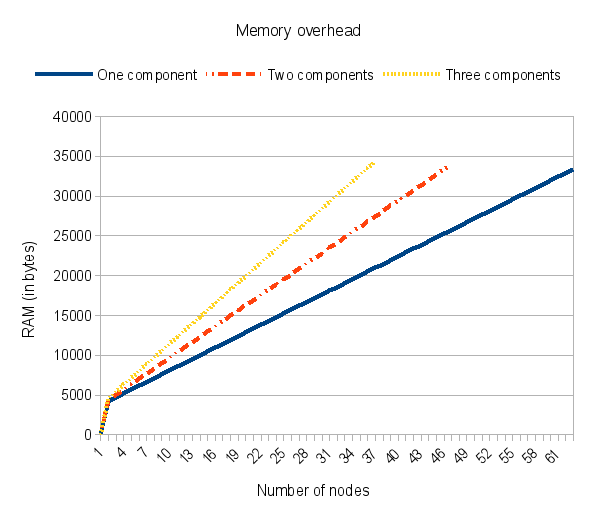
\includegraphics[width=0.7\columnwidth]{chapters/modelsAtRuntimeContiki.images/MemoryOverhead3Nodes.png}
	\caption{Memory overhead for 1, 2 and 3 \emph{Blink/COAP} components.} \label{fig:MemUsedBlinkComps}
\end{figure}


Figure \ref{fig:MemUsedBlinkComps} shows the memory usage for each model depending on its size.
These results show that our current implementation enables to scale the model up to 60 nodes with one component per node, and up to 37 nodes with three components per node. These numbers are encouraging, since some tens of nodes could enable IoT systems and IoT devices to run in various environments like house, building, car, factory chain etc.

\subsection{Summary}
\todo{consider the model size for the next contribution}

Our initial results show that the models@runtime implementation is feasible for IoT devices and there are enough resources to deploy several other functional software components.
It is possible to observe that our overheads are small enough to affect the overall operation of a node, while adding an abstract representation of the running system, in addition to reconfiguration and adaptation features.
Since these results are promising, we showed that our middleware is able to manipulate a running application by affecting it through a component model, without an important overhead, neither in memory nor in energy consumption.

As a final consideration, the executed application contained a very minimalistic model, including only enough characteristics to manipulate such model.
Indeed, for the next chapter, a more complete implementation of the modeling framework is proposed, resulting in a more robust middleware.
For this reason, the size of the application can increase, and the ability to instantiate components and nodes at the model level can be decreased.

Several challenges were raised with the results of this first approach.
The first one, lies in the way that the model should be spread across the network.
Since the same model should be present in all the nodes forming the network, we must investigate epidemic algorithms of distribution.
The second one is about the creation of components and its distribution across the nodes.
Special attention is being put on this last feature.
Distributing software components on mesh topologies, which are less robust than typical computer networks, raise scientific questions about the best method to provide them.
Thus, a distributed algorithm to download components taking into account the network topology and energy consumption should be proposed.

The next chapter will describe our contributions that propose answers to that questions. 